\documentclass[a4]{article}
\usepackage{graphicx}
\usepackage{titlesec}
\thispagestyle{empty}
\topmargin=0.0in
\topmargin=0.0in
\headheight=0pt
\headsep=0pt
\oddsidemargin=0.0in
\evensidemargin=0in
\marginparwidth=0in
\textwidth=6.2in
\textheight=9.5in
\begin{document}
\setlength{\parindent}{0em}


\titleformat{\subsection}
{\bfseries}
{$\bullet$}
{0em}
{}

%Name on top
\centerline{
\textsc{\LARGE Kunal Kishore Sahu}
}

%vertical space and horizontal rule after name
\vspace{5mm}
\hrule
\vspace{2mm}

%personal information
Kamal Nivas,Shaktinagar 2nd lane \hspace{7.4cm} Contact: 7381589522\\
Berhampur, \hspace{9cm} E-mail ID: ksahu2076@gmail.com\\
Odisha-760001

%photograph
\begin{figure}[h!]
\hspace{10.5cm}
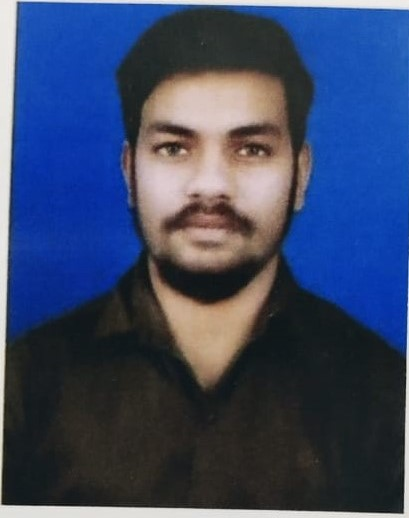
\includegraphics[height=2cm]{resume_pic}
\end{figure}

%objective
\vspace{3mm}
\textbf{OBJECTIVE : }
To secure a position where I can effectively use my skills and apply my knowledge in practical use for the growth of organization and for public welfare.


%education
\vspace{5mm}
\textbf{EDUCATION : } 
\vspace{1mm} \\

\begin{tabular}{|c|c|c|c|c|}

\hline
\textbf{Degree} & \textbf{College/School} & \textbf{University/Board} & \textbf{Passing Year} & \textbf{Passing Percentage} \\
\hline
B.Tech. & NIST, Berhampur & BPUT & 2020 & - \\
\hline
Intermediate & Kendriya Vidyalaya Berhampur & CBSE & 2016 & 75 \\
\hline
Matriculation & Kendriya Vidyalaya Berhampur & CBSE & 2014 & 93 \\
\hline

\end{tabular}


%projects
\vspace{3mm}
\textbf{Projects : } 
\begin{enumerate}
	\item Fully Autonomous Line Follower using PID algorithm ,which can detect different colors and sound frequencies 
and traverse its path, NSSC- ISRO,IIT kharagpur,10/2018. 
	\item Simulation of Smart traffic light using 8051 microcontroller in Proteus-certification project, CTTC, 
Bhubaneswar,06/2018.
         \item PWM circuit, SPHO, BPUT, 03/2018. 
         \item Dual Axis Solar Tracker without using microcontroller, Sankalp,NIST,Berhampur 02/2018.
         \item Smart Museum, monitoring different parameters-temperature, humidity, quality of air, date, time and real time 
Data logging ,Sankalp ,NIST,Berhampur,02/201.
         \item Built a robot and a lift mechanism to pick and deposit the nuts at designated zones using path planning algorithm to deposit
the nuts at deposit zones, e-YRC-2018 , IIT-Bombay , 29/03,2019.
\end{enumerate}

%trainings and internships
\vspace{3mm}
\textbf{TRAINING AND INTERNSHIP : } 
\begin{itemize}
	\item Certification course on Embedded systems , at CTTC, Bhubaneswar, 01/06
/2018 -31/06/2018 .
	\item Certification course on Programmable Logic Controller , at CTTC,Bhubaneswar, 01/06
/2018-31/06/2018 .
         \item British English Council- Certified -Preliminary,07/2017. 
         \item Attended 1 day Workshop on Internet of Things(IoT), at IIT-Kharagpur, by Robonext 07/2017 .
         \item Certification course on Introduction to Oracle 11g:SQL  at, NIST, Berhampur, 
05/2017 .
\end{itemize}

%technical skills
\vspace{3mm}
\textbf{TECHNICAL SKILLS : } 

\subsection{Simulation Softwares}	
      PSPICE, TINA, Microsoft Office, Proteus
\subsection{Programming Languages}
 C, C++
\subsection{Others}
Arduino , Keil Microvision , Latex , Atmel Studio , Oracle 11g


\end{document}